\subsection{Presentation interface}

The concept of this interface is to keep the user from accessing their devices, just to check to current playlist configuration but instead provide quick and easely accessicible overview for the users of the system, bargoers and administrator both. By having seperated screen from the users devices, the system may reduce the amount of time spent using the devices which was declared a problem best seen minimized, as an effect of the system, concluded in \cref{sub:user_requirements}. The intention is to have the playlist on a screen above the bar, as visually envisioned in \cref{fig:PresentationInterface}. This should direct the users eyes towards the bar, if they are interested in viewing the current results, by making it more accesible to the user as the screen being bigger in size and always on opposed to the small handheld device\cite{DEB}. It is important to stress that the screen should not be visually blockable by person or other objects though, by placing the just under the roof. 
This is a part of the system which is always visually accessible for the user, therefore should also be visually pleasing to look at, but still contain all the information needed by the user. An interesting problem to solve is have to diplay each individuals votes in an efficient way, without providing an overflood of information, confusing the user instead. One solution suggest is to have to the most distinguishing content to the left with the reading direction, and the least distinguishing content to the right\cite{material}. In this case a tracks placement(1,2,3...) on the playlist to the left and the users who voted for it on the right. Depicting the user will require some sort of id, through a login or similar, to recognise a specific users from others.

\begin{figure}[H]
  \centering
  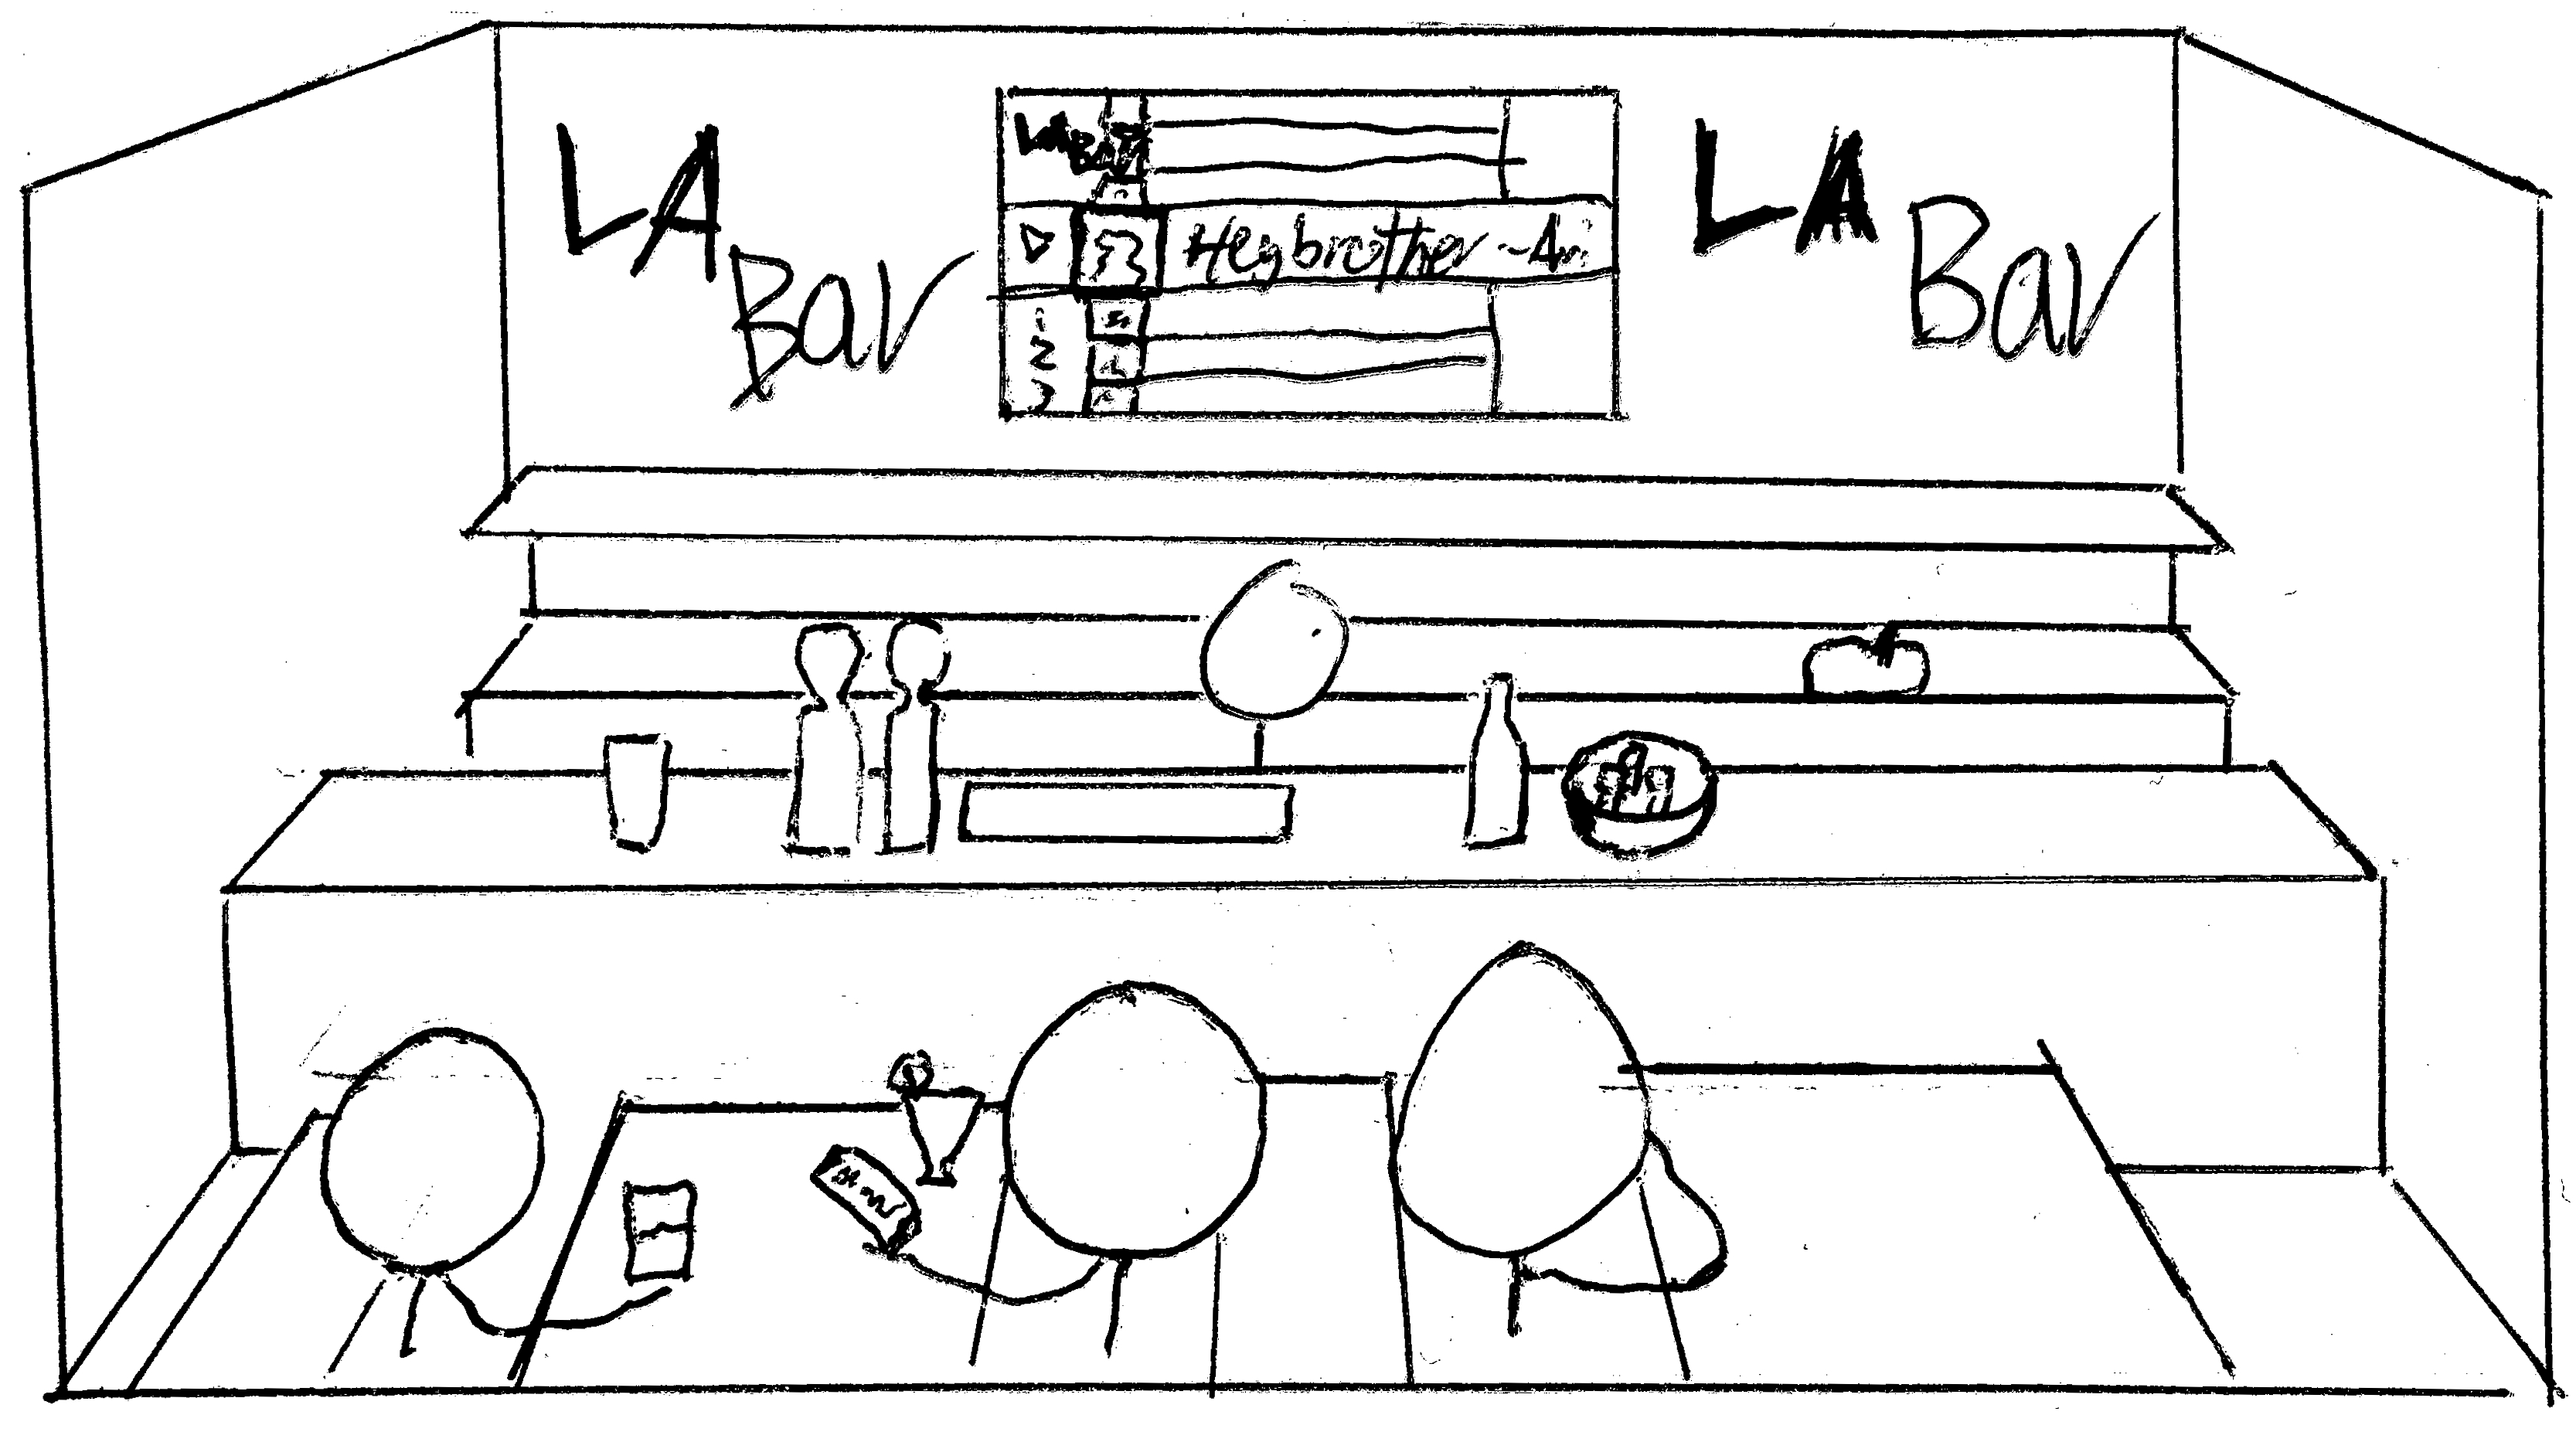
\includegraphics[width=1.0\linewidth]{Images/presentation.png}
  \caption{Sketch of the screen in context and visual design}\label{fig:PresentationInterface}
\end{figure}